% ══════════════════════════════════════════════════════════════════════════════
%  ADVANCED SEPARATION — the above-level book (from 2027)
%  Faculty decision, Nov 2026: every student completes the at-level lesson books;
%  students who excel move on to this book. Its topics go deeper into the ideas
%  of the at-level lessons rather than adding more of the same work.
%
%  Each topic: a reading, the deeper idea worked through (I do / We do), then
%  %%PARTD:N%% pulls in the old Part D questions of at-level Lesson N (the
%  unit's lesson numbers) as practice, then a Challenge.
%  Built by make_a5.py (via a5_levels.py).
% ══════════════════════════════════════════════════════════════════════════════

% ══════════════════════════════════════════════════════════════════════════════
%  TOPIC 1 — ATOMS, ELEMENTS AND COMPOUNDS               (deepens Lessons 1, 4)
% ══════════════════════════════════════════════════════════════════════════════
\setcounter{section}{0}\renewcommand{\lessonart}{16}
\sectiondiv{Atoms, Elements and Compounds}{Dalton's atoms \textbullet{} The periodic table \textbullet{} Reading a formula \textbullet{} Why compounds are not mixtures}\label{sec:1}
\lessoncodes{Deepens Lessons 1 and 4 \textbullet{} VC2S8U07 \textbullet{} VC2S10U07}

\vocabhead
\begin{ctab}
\begin{tabular}{|SW{3.4cm}|W{7.0cm}|}
  \hline\hd & \thead{Word} & \thead{Definition (copy from the slide)} \\ \hline
  & \scaf{\textbf{Atom}} & \scaf{The smallest particle of an element.} \\ \hline
  & \textbf{Periodic table} & \\ \hline
  & \textbf{Chemical symbol} & \\ \hline
  & \textbf{Chemical formula} & \\ \hline
  & \textbf{Fixed ratio} & \\ \hline
\end{tabular}
\end{ctab}

\lessonpart{A}{Reading and comprehension}{Teal}\label{read:1}

\begin{readingbox}{Reading --- A Table With Gaps}
In 1808 the English teacher John Dalton argued that every element is made of its own kind of tiny, solid \textbf{atom}, and that compounds form when atoms of different elements join in simple whole-number ratios. Water, he said, is always the same combination, wherever it comes from. Experiments kept agreeing with him.

Scientists found more and more elements, and each was given a one- or two-letter \textbf{chemical symbol}: H for hydrogen, O for oxygen, Na for sodium (from its Latin name, \emph{natrium}). In 1869 the Russian chemist Dmitri Mendeleev arranged the 63 known elements in order of the mass of their atoms, in rows, so that elements with similar properties lined up in columns. Where the pattern did not fit, he left gaps, and predicted that new elements would be found to fill them. Within twenty years gallium and germanium were discovered, with almost exactly the properties he had predicted. His arrangement became the \textbf{periodic table}, which now holds 118 elements.

A \textbf{chemical formula} shows which atoms are joined in one particle of a compound, and how many of each. Because the atoms are always joined in the same \textbf{fixed ratio}, a compound always has the same make-up, unlike a mixture, which can be mixed in any proportion.
\end{readingbox}

\rcreset
\rcq{What were two of Dalton's ideas about atoms and compounds?}{2.5cm}
\rcq{Why did Mendeleev leave gaps in his table, and why was that a bold thing to do?}{3cm}
\rcq{Why is the symbol for sodium Na and not S?}{2cm}
\rcq{How is the make-up of a compound different from the make-up of a mixture?}{2.5cm}

\lessonpart{B}{Theory and examples}{Blue}\label{theory:1}

\subsection{Reading a Formula}\label{sub:a1.1}

\begin{skillbox}{Formulas}
Each capital letter starts a new element. A small number after a symbol counts the atoms of that element; no number means one. \quad H\textsubscript{2}O: 2 hydrogen, 1 oxygen.
\end{skillbox}

\begin{workedex}{Glucose, C\textsubscript{6}H\textsubscript{12}O\textsubscript{6}}
Carbon: 6 atoms. Hydrogen: 12. Oxygen: 6.\\
That is \textbf{3 elements} and $6 + 12 + 6 = \mathbf{24}$ atoms in each particle of glucose.
\end{workedex}

\begin{wedo}{Counting atoms}
For each compound, name the elements and count the atoms in one particle: ammonia, NH\textsubscript{3}; sulfuric acid, H\textsubscript{2}SO\textsubscript{4}; calcium carbonate (chalk), CaCO\textsubscript{3}.
\answerbox{5cm}
\end{wedo}

\subsection{A Compound Is Not a Mixture}\label{sub:a1.2}

\begin{workedex}{Table salt}
Sodium is a soft, shiny metal that fizzes violently in water. Chlorine is a poisonous green gas. Joined, they make sodium chloride, NaCl: table salt, which we eat every day.

\smallskip
A compound has \textbf{new properties}, unlike either element, and the atoms are joined in a fixed ratio (one sodium to one chlorine). In a mixture, each part keeps its own properties and can be in any proportion.
\end{workedex}

\begin{wedo}{Water}
Hydrogen is a gas that burns explosively. Oxygen is a gas that makes things burn more fiercely. Explain how water shows that it is a compound and not a mixture of these two gases. Give two pieces of evidence.
\answerbox{5cm}
\end{wedo}

\lessonpart{C}{Practice}{Amber}\label{prac:1}

%%PARTD:1%%

%%PARTD:4%%

\lessonpart{D}{Challenge}{Violet}\label{ext:1}

\task Every 18\,g of pure water, from anywhere, contains 2\,g of hydrogen and 16\,g of oxygen.
\pt{a} How much hydrogen and how much oxygen are in 45\,g of water? Show your working.
\workbox{4cm}
\pt{b} A container of hydrogen and oxygen \emph{gases} can hold the two in any ratio. Explain why water cannot, using the idea of atoms joined in a fixed ratio.
\answerbox{4.5cm}

\clearpage

% ══════════════════════════════════════════════════════════════════════════════
%  TOPIC 2 — MIXTURES BY NUMBERS                         (deepens Lessons 2, 5)
% ══════════════════════════════════════════════════════════════════════════════
\setcounter{section}{1}\renewcommand{\lessonart}{19}
\sectiondiv{Mixtures by Numbers}{Concentration in g/L \textbullet{} Dilution \textbullet{} Very small amounts: parts per million}\label{sec:2}
\lessoncodes{Deepens Lessons 2 and 5 \textbullet{} VC2S8U06 \textbullet{} VC2S10I04}

\vocabhead
\begin{ctab}
\begin{tabular}{|SW{3.4cm}|W{7.0cm}|}
  \hline\hd & \thead{Word} & \thead{Definition (copy from the slide)} \\ \hline
  & \scaf{\textbf{Concentration}} & \scaf{How much solute is dissolved in a given volume of solution.} \\ \hline
  & \textbf{Grams per litre (g/L)} & \\ \hline
  & \textbf{Dilute (verb)} & \\ \hline
  & \textbf{Percentage by mass} & \\ \hline
  & \textbf{Parts per million (ppm)} & \\ \hline
\end{tabular}
\end{ctab}

\lessonpart{A}{Reading and comprehension}{Teal}\label{read:2}

\begin{readingbox}{Reading --- How Much Is in There?}
``Strong'' and ``weak'' are fine words in the kitchen, but a chemist, a nurse or a water engineer needs numbers. The \textbf{concentration} of a solution says how much solute is in a set volume of it. One common unit is \textbf{grams per litre} (g/L): the mass of solute in every litre of solution. Sea water is about 35\,g/L of salt.

To \textbf{dilute} a solution, you add more solvent. The amount of solute does not change, but it is spread through a bigger volume, so the concentration falls. Cordial, cleaning products and medicines are all diluted before use, and the instructions are written so the right concentration is reached.

Mixtures of solids are often described by \textbf{percentage by mass}: 18-carat gold is 75\% gold by mass. For very small amounts, scientists use \textbf{parts per million} (ppm). One ppm is one gram of something in a million grams of mixture, or about one milligram in a litre of water. Melbourne's tap water has fluoride added at about 1\,ppm to protect teeth; drinking-water rules limit lead to less than 0.01\,ppm.
\end{readingbox}

\rcreset
\rcq{Why do scientists describe concentration with numbers instead of ``strong'' or ``weak''?}{2.5cm}
\rcq{What stays the same, and what changes, when a solution is diluted?}{2.5cm}
\rcq{What does 1\,ppm mean?}{2cm}
\rcq{Why is ppm a better unit than g/L for the lead in drinking water?}{2.5cm}

\lessonpart{B}{Theory and examples}{Blue}\label{theory:2}

\subsection{Concentration in g/L}\label{sub:a2.1}

\begin{skillbox}{Concentration}
\[ \text{concentration (g/L)} = \frac{\text{mass of solute (g)}}{\text{volume of solution (L)}} \qquad 1\,\text{L} = 1000\,\text{mL} \]
\end{skillbox}

\begin{workedex}{Sugar in water}
25\,g of sugar is dissolved to make 500\,mL of solution.

\smallskip
$500\,\text{mL} = 0.5\,\text{L}$. \quad Concentration $= 25 \div 0.5 = \mathbf{50\ g/L}$.
\end{workedex}

\begin{wedo}{A sports drink}
A 600\,mL bottle of sports drink contains 36\,g of sugar. Find its concentration in g/L. Is it more or less concentrated than the worked example?
\workbox{4cm}
\end{wedo}

\subsection{Dilution}\label{sub:a2.2}

\begin{workedex}{Making up cordial}
200\,mL of cordial with a sugar concentration of 100\,g/L is topped up with water to 1\,L. Find the new concentration.

\smallskip
Sugar in the cordial: $100 \times 0.2 = 20$\,g. Diluting does not change this.\\
New concentration $= 20 \div 1 = \mathbf{20\ g/L}$: five times the volume, one-fifth the concentration.
\end{workedex}

\begin{wedo}{Diluting salt water}
50\,mL of salt water at 40\,g/L is diluted to 250\,mL. Find the mass of salt and the new concentration.
\workbox{4.5cm}
\end{wedo}

\lessonpart{C}{Practice}{Amber}\label{prac:2}

%%PARTD:2%%

%%PARTD:5%%

\lessonpart{D}{Challenge}{Violet}\label{ext:2}

\task Melbourne's tap water contains about 1\,ppm of fluoride, that is, about 1\,mg in each litre.
\pt{a} A student drinks 2\,L of tap water a day. How many milligrams of fluoride is that in a year? Give your answer in grams too. (1\,g $=$ 1000\,mg.)
\workbox{4cm}
\pt{b} A dentist says the amount is safe and helps teeth, but much more would harm them. Explain why it matters that the water authority measures and controls the concentration, not just whether fluoride is present.
\answerbox{4.5cm}

\clearpage

% ══════════════════════════════════════════════════════════════════════════════
%  TOPIC 3 — SEPARATING BY SIZE, DENSITY AND MAGNETISM       (deepens Lesson 7)
% ══════════════════════════════════════════════════════════════════════════════
\setcounter{section}{2}\renewcommand{\lessonart}{25}
\sectiondiv{Separating by Size, Density and Magnetism}{Choosing a method from a property \textbullet{} Separating in several steps \textbullet{} Sedimentation and the centrifuge}\label{sec:3}
\lessoncodes{Deepens Lesson 7 \textbullet{} VC2S8U06 \textbullet{} VC2S10H02}

\vocabhead
\begin{ctab}
\begin{tabular}{|SW{3.4cm}|W{7.0cm}|}
  \hline\hd & \thead{Word} & \thead{Definition (copy from the slide)} \\ \hline
  & \scaf{\textbf{Sedimentation}} & \scaf{Letting heavier, denser solid particles settle to the bottom of a liquid.} \\ \hline
  & \textbf{Sediment} & \\ \hline
  & \textbf{Centrifuge} & \\ \hline
  & \textbf{Sieve} & \\ \hline
  & \textbf{Flocculant} & \\ \hline
\end{tabular}
\end{ctab}

\lessonpart{A}{Reading and comprehension}{Teal}\label{read:3}

\begin{readingbox}{Reading --- From River to Tap}
Water from a reservoir carries fine clay and silt that would take weeks to settle. At a water treatment plant, a \textbf{flocculant} is stirred in. It makes the tiny particles clump into larger, heavier flakes. In big settling tanks the flakes sink: this is \textbf{sedimentation}, and the layer that forms on the bottom is the \textbf{sediment}. The clearer water above flows over the top, then through filters of sand and gravel.

When a mixture will not settle quickly enough, scientists spin it. A \textbf{centrifuge} whirls test tubes around hundreds of times a second. The spinning acts like extra-strong gravity, so the denser parts are flung to the bottom in minutes. A blood sample spun in a centrifuge separates into a layer of red cells at the bottom and pale yellow plasma on top. Dairies use the same idea to separate cream from milk.

Many real mixtures need several steps. A \textbf{sieve} sorts by particle size, a magnet removes iron and steel, water dissolves what is soluble, and density lets light and heavy parts be washed or spun apart. Engineers choose the order so each step leaves an easier mixture for the next.
\end{readingbox}

\rcreset
\rcq{What does a flocculant do, and why does it make sedimentation faster?}{2.5cm}
\rcq{Why does spinning in a centrifuge separate a mixture faster than leaving it to settle?}{2.5cm}
\rcq{Describe what a blood sample looks like after it has been spun.}{2cm}
\rcq{Why must engineers think about the order of the steps?}{2.5cm}

\lessonpart{B}{Theory and examples}{Blue}\label{theory:3}

\subsection{Choosing a Method from a Property}\label{sub:a3.1}

\begin{ctab}
\begin{tabular}{|W{3.6cm}|W{6.6cm}|}
  \hline\thead{Property that differs} & \thead{Methods that use it} \\ \hline
  Particle size & sieving, filtering \\ \hline
  Density & decanting, sedimentation, centrifuging, panning \\ \hline
  Magnetism & magnetic separation \\ \hline
  Solubility & dissolving, then filtering \\ \hline
  Boiling point & evaporation, distillation \\ \hline
\end{tabular}
\end{ctab}

\begin{workedex}{Sand, iron filings and salt}
\textbf{1.} Draw a magnet through the dry mixture: the iron filings stick to it (magnetism). \textbf{2.} Stir the rest into water: the salt dissolves, the sand does not (solubility). \textbf{3.} Filter: the sand is the residue (particle size). \textbf{4.} Evaporate the filtrate: salt is left (boiling point).
\end{workedex}

\begin{wedo}{Four ingredients}
A mixture contains rice grains, sand, salt and iron filings. Plan the steps to separate all four, in order. For each step, name the property it uses.
\answerbox{6cm}
\end{wedo}

\subsection{Sedimentation and the Centrifuge}\label{sub:a3.2}

\begin{workedex}{Muddy water}
Muddy water is left in a jar. After an hour the sand has settled but the water is still cloudy. Explain.

\smallskip
Sand grains are large and dense, so they sink quickly. The clay particles are so tiny that the water's moving particles keep bumping them around, and they sink extremely slowly. A flocculant, a filter or a centrifuge would be needed to clear the water.
\end{workedex}

\begin{wedo}{Spinning blood}
After a blood sample is spun, the red cells are at the bottom and the plasma at the top. Which part is denser? Explain why a hospital spins blood instead of leaving it to settle.
\answerbox{4.5cm}
\end{wedo}

\lessonpart{C}{Practice}{Amber}\label{prac:3}

%%PARTD:7%%

\lessonpart{D}{Challenge}{Violet}\label{ext:3}

\task A recycling plant receives a crushed mixture of steel, aluminium, glass and paper. Design a flow chart of steps to separate all four. For each step, name the method and the property it uses, and explain why your order works.
\answerbox{9cm}

\clearpage

% ══════════════════════════════════════════════════════════════════════════════
%  TOPIC 4 — CRYSTALS AND SOLUBILITY CURVES          (deepens Lessons 8, 10, 12)
% ══════════════════════════════════════════════════════════════════════════════
\setcounter{section}{3}\renewcommand{\lessonart}{21}
\sectiondiv{Crystals and Solubility Curves}{Reading a solubility curve \textbullet{} How much crystallises? \textbullet{} Big crystals, small crystals \textbullet{} Purifying by recrystallisation}\label{sec:4}
\lessoncodes{Deepens Lessons 8, 10 and 12 \textbullet{} VC2S8U06 \textbullet{} VC2S10I05}

\vocabhead
\begin{ctab}
\begin{tabular}{|SW{3.4cm}|W{7.0cm}|}
  \hline\hd & \thead{Word} & \thead{Definition (copy from the slide)} \\ \hline
  & \scaf{\textbf{Solubility curve}} & \scaf{A graph of how much solute dissolves in 100\,g of water at each temperature.} \\ \hline
  & \textbf{Crystal lattice} & \\ \hline
  & \textbf{Recrystallisation} & \\ \hline
  & \textbf{Impurity} & \\ \hline
  & \textbf{Rate of cooling} & \\ \hline
\end{tabular}
\end{ctab}

\lessonpart{A}{Reading and comprehension}{Teal}\label{read:4}

\begin{readingbox}{Reading --- Slow Cooling, Big Crystals}
Look closely at salt or sugar and you will see tiny cubes and blocks with flat faces. Their shape comes from the way the particles stack in a regular, repeating pattern called a \textbf{crystal lattice}. As a solution cools or evaporates, particles join the lattice one layer at a time.

How big the crystals grow depends on the \textbf{rate of cooling}. Cool a solution slowly and particles have time to find their places on a few growing crystals, so they become large. Cool it fast and many tiny crystals start at once. The same is true of rocks: granite cooled slowly deep underground and has crystals you can see; basalt cooled quickly at the surface and its crystals are tiny.

Factories use crystals to make substances purer. Raw sugar is dissolved in hot water, filtered, and cooled. The sugar crystallises out, while most of the \textbf{impurities}, being only a small amount, stay dissolved. This is \textbf{recrystallisation}. A \textbf{solubility curve} tells chemists exactly how much will crystallise at each temperature.
\end{readingbox}

\rcreset
\rcq{What gives a crystal its flat faces and regular shape?}{2.5cm}
\rcq{Why does slow cooling make larger crystals?}{2.5cm}
\rcq{Explain why granite and basalt have different crystal sizes.}{2.5cm}
\rcq{Why do the impurities stay in solution during recrystallisation?}{2.5cm}

\lessonpart{B}{Theory and examples}{Blue}\label{theory:4}

\subsection{How Much Crystallises?}\label{sub:a4.1}

\begin{center}
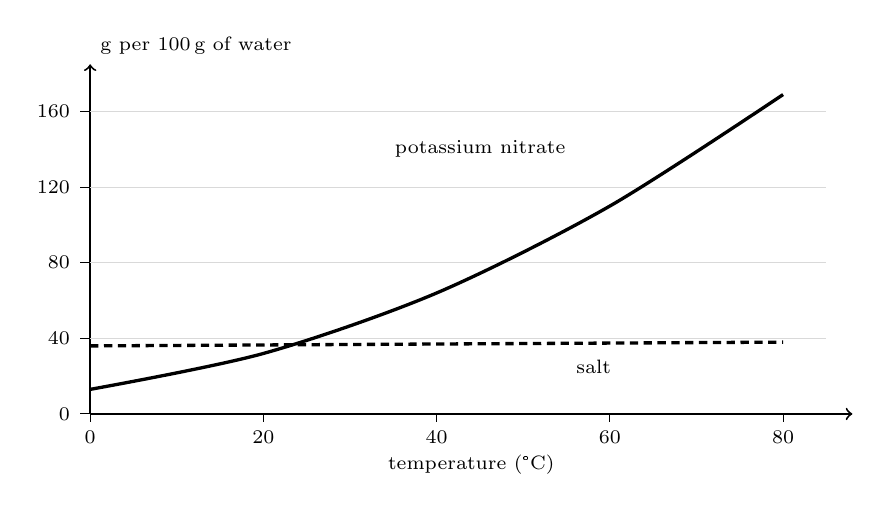
\begin{tikzpicture}[font=\small, x=0.11cm, y=0.024cm]
  \draw[->, line width=0.7pt] (0,0) -- (88,0) node[pos=0.5, below=11pt, font=\scriptsize] {temperature (\textdegree C)};
  \draw[->, line width=0.7pt] (0,0) -- (0,185) node[above right, font=\scriptsize] {g per 100\,g of water};
  \foreach \x in {0,20,40,60,80} \draw (\x,0) -- (\x,-4) node[below, font=\scriptsize] {\x};
  \foreach \y in {0,40,80,120,160} \draw (0,\y) -- (-1.2,\y) node[left, font=\scriptsize] {\y};
  \foreach \y in {40,80,120,160} \draw[black!15] (0,\y) -- (85,\y);
  \draw[line width=1.2pt] plot[smooth] coordinates {(0,13) (20,32) (40,64) (60,110) (80,169)};
  \node[font=\scriptsize, anchor=east] at (56,140) {potassium nitrate};
  \draw[line width=1.2pt, densely dashed] (0,36) -- (80,38);
  \node[font=\scriptsize, anchor=west] at (55,25) {salt};
\end{tikzpicture}
\figcap{Solubility of potassium nitrate (solid) and salt (dashed).}
\end{center}

\begin{workedex}{Cooling a saturated solution}
100\,g of water is saturated with potassium nitrate at 60\,\textdegree C and cooled to 20\,\textdegree C. What mass of crystals forms?

\smallskip
At 60\,\textdegree C it holds 110\,g; at 20\,\textdegree C only 32\,g. The rest comes out as crystals: $110 - 32 = \mathbf{78\ g}$.
\end{workedex}

\begin{wedo}{Half the water}
50\,g of water is saturated with potassium nitrate at 40\,\textdegree C and cooled to 20\,\textdegree C. Use the graph to find the mass of crystals. (Hint: 50\,g of water holds half as much as 100\,g.)
\workbox{5cm}
\end{wedo}

\subsection{Big Crystals, Small Crystals}\label{sub:a4.2}

\begin{workedex}{Rock candy}
Sugar syrup left on a windowsill for a week grows large crystals on a string. The same syrup put in a freezer forms a grainy paste of tiny crystals. Explain.

\smallskip
On the windowsill water evaporates slowly, so sugar particles join a few crystals one by one and they grow large. In the freezer the syrup cools quickly, so crystals start in thousands of places at once and none can grow big.
\end{workedex}

\begin{wedo}{Two igneous rocks}
Rock X has crystals several millimetres across; rock Y looks smooth, with crystals too small to see. Both formed from the same molten rock. Which cooled underground and which in a lava flow? Explain.
\answerbox{4.5cm}
\end{wedo}

\lessonpart{C}{Practice}{Amber}\label{prac:4}

%%PARTD:8%%

%%PARTD:10%%

%%PARTD:12%%

\lessonpart{D}{Challenge}{Violet}\label{ext:4}

\task A sample of potassium nitrate is contaminated with sand and a small amount of salt. Using the solubility curve, plan a method to get pure, dry potassium nitrate crystals. Give the temperatures you would use, explain how each step removes one of the impurities, and say why a little potassium nitrate will always be lost.
\answerbox{9cm}

\clearpage

% ══════════════════════════════════════════════════════════════════════════════
%  TOPIC 5 — DISTILLATION AND CHROMATOGRAPHY AT WORK        (deepens Lesson 16)
% ══════════════════════════════════════════════════════════════════════════════
\setcounter{section}{4}\renewcommand{\lessonart}{27}
\sectiondiv{Distillation and Chromatography at Work}{Fractional distillation \textbullet{} Oil refineries and liquid air \textbullet{} $R_f$ values in forensic science \textbullet{} Making fresh water}\label{sec:5}
\lessoncodes{Deepens Lesson 16 \textbullet{} VC2S8U06 \textbullet{} VC2S10H02 \textbullet{} VC2S10H03}

\vocabhead
\begin{ctab}
\begin{tabular}{|SW{3.4cm}|W{7.0cm}|}
  \hline\hd & \thead{Word} & \thead{Definition (copy from the slide)} \\ \hline
  & \scaf{\textbf{Fractional distillation}} & \scaf{Separating a mixture of liquids with different boiling points, using a tall column, into parts called fractions.} \\ \hline
  & \textbf{Fraction} & \\ \hline
  & \textbf{Crude oil} & \\ \hline
  & \textbf{$R_f$ value} & \\ \hline
  & \textbf{Reverse osmosis} & \\ \hline
\end{tabular}
\end{ctab}

\lessonpart{A}{Reading and comprehension}{Teal}\label{read:5}

\begin{readingbox}{Reading --- Separating on a Giant Scale}
\textbf{Crude oil} pumped from the ground is a thick, dark mixture of hundreds of substances. At a refinery it is heated until most of it boils, and the vapour rises up a tower many storeys tall that is hot at the bottom and cooler at the top. Each substance condenses back into a liquid at the height where the tower is cool enough for it. Trays at different heights collect each \textbf{fraction}: gases for cooking at the top, then petrol, kerosene for jet fuel, diesel, and thick bitumen for roads at the bottom. This is \textbf{fractional distillation}.

The air you breathe is separated the same way, but the other way round: air is cooled to about $-200$\,\textdegree C until it becomes a liquid, and then allowed to warm. Nitrogen boils off first, at $-196$\,\textdegree C, then oxygen at $-183$\,\textdegree C. Hospitals use the oxygen.

Chromatography works on tiny samples. Forensic scientists use it to match an ink to a pen, and sports drug testers use it to find banned substances in a drop of urine. Each substance travels a set fraction of the distance the solvent travels, its \textbf{$R_f$ value}, so it can be identified like a fingerprint.

Victoria's desalination plant at Wonthaggi does not distil sea water. It uses \textbf{reverse osmosis}: sea water is pushed at high pressure through a membrane whose pores let water particles through but hold the salt back.
\end{readingbox}

\rcreset
\rcq{Why does each fraction collect at a different height in the tower?}{2.5cm}
\rcq{In which order do nitrogen and oxygen boil off as liquid air warms? Why?}{2.5cm}
\rcq{Give two uses of chromatography outside a school lab.}{2cm}
\rcq{How does reverse osmosis separate salt from water?}{2.5cm}

\lessonpart{B}{Theory and examples}{Blue}\label{theory:5}

\subsection{Fractional Distillation}\label{sub:a5.1}

\begin{workedex}{Three liquids}
A mixture contains pentane (boils at 36\,\textdegree C), hexane (69\,\textdegree C) and heptane (98\,\textdegree C). It is heated slowly in a fractionating column. In what order are they collected?

\smallskip
The lowest boiling point boils first and reaches the top of the column: \textbf{pentane}, then \textbf{hexane}, then \textbf{heptane}. The thermometer stays near 36\,\textdegree C while pentane distils, then rises towards 69\,\textdegree C.
\end{workedex}

\begin{wedo}{Liquid air}
Liquid air contains nitrogen (boils at $-196$\,\textdegree C), argon ($-186$\,\textdegree C) and oxygen ($-183$\,\textdegree C). In what order do they boil off as it warms? Explain why argon and oxygen are the hardest pair to separate.
\answerbox{4.5cm}
\end{wedo}

\subsection{$R_f$ Values}\label{sub:a5.2}

\begin{skillbox}{$R_f$ value}
\[ R_f = \frac{\text{distance moved by the spot}}{\text{distance moved by the solvent front}} \]
Both distances are measured from the starting line. The same substance, with the same paper and solvent, always has the same $R_f$.
\end{skillbox}

\begin{workedex}{Matching a dye}
A spot moved 2.4\,cm while the solvent front moved 6.0\,cm. $R_f = 2.4 \div 6.0 = \mathbf{0.40}$. Known dyes: yellow 0.25, red 0.40, blue 0.70. The spot is the \textbf{red} dye.
\end{workedex}

\begin{wedo}{A forged signature}
Ink from a forged cheque gave two spots, 1.5\,cm and 4.8\,cm from the start, with the solvent front at 6.0\,cm. Pen P's ink has spots with $R_f$ 0.25 and 0.80; pen Q's has 0.25 and 0.60. Which pen was used? Show your working.
\workbox{5cm}
\end{wedo}

\lessonpart{C}{Practice}{Amber}\label{prac:5}

%%PARTD:16%%

\lessonpart{D}{Challenge}{Violet}\label{ext:5}

\task A remote island has plenty of sunshine and sea water, but no electricity grid and little fuel. Compare distillation and reverse osmosis as ways to make its drinking water: what each needs, and its advantages and disadvantages. Recommend one, and justify your choice.
\answerbox{9cm}

\clearpage
